\chapter{提案手法}
本章ではGCNを欠損値データに適用するための欠損値補完を用いた2つの手法を提案する。

\section{構造的補完}
\label{sec:structurally_imputation}
\begin{figure*}[h]
  \centering
  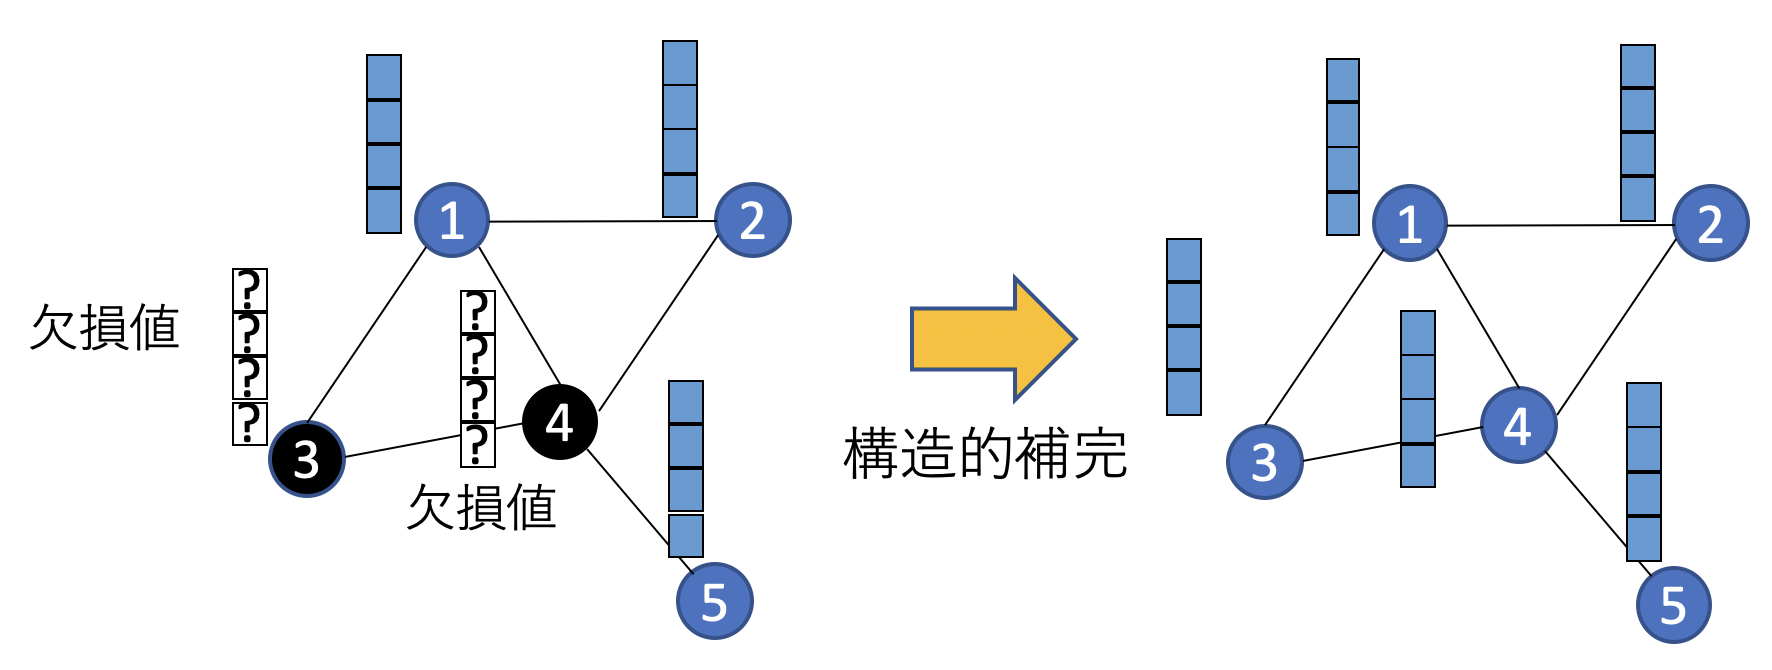
\includegraphics[width=1\hsize]{figures/structurally_imputation.png}
  \caption{構造的補完}
  \label{fig:structurally_imputation}
\end{figure*}
欠損値を代入法を用いて補完する手法のうち、グラフ構造を用いて欠損値補完をする手法を構造的補完と定義する。図\ref{fig:structurally_imputation}は構造的補完の例を示している。この図では便宜的にノードの全ての特徴量が欠損しているノードと特徴量の全てが欠損していないノードの2種類のノードから成り立つグラフを用いている。図\ref{fig:structurally_imputation}の左図はノード番号3と4のノードの特徴量が全て欠損しており、ノード番号1,2,5のノードの特徴量は欠損していないケースを示している。図\ref{fig:structurally_imputation}の左図に構造的補完を適用することで右図のように全てのノードに欠損値のないグラフを得ることができる。構造的補完により求められる欠損値を補完された特徴量$X'_{ij}$は以下の式\eqref{eq:structurally_imputation}のように定義できる。
\begin{align} \label{eq:structurally_imputation}
    X'_{ij} =
    \begin{cases}
      X_{ij}&  (r_{ij} = 1) \\
      F(X_{ij},A)  & (r_{ij} = 0)
    \end{cases}
\end{align}

ここで$X_{ij}$は欠損値を含む特徴量、$A$は隣接行列、$F$は構造的補完の方法により決まる関数である。$r_{ij}$は$x_{ij}$が観測値の場合には1で$x_{ij}$が欠損値の場合には0と定義する。

\section{近隣平均補完}
本節では提案手法で用いる近隣平均補完について述べる。近隣平均補完は構造的補完の1つであり、特徴量の種類ごとに欠損値補完を行う手法である。欠損しているノードの特徴量を、そのノードの近隣ノードのうち欠損していないノードの特徴量の平均を用いて補完する方法を近隣平均補完と定義する。またもしそのノードの近隣ノードの全てが欠損値を含んでいる場合は0を特徴量として代入する。近隣平均補完により求められる欠損値を補完された特徴量$X'_{ij}$は以下の式\eqref{eq:neighbor_imputation}のように定義できる。
\begin{align} \label{eq:neighbor_imputation}
    X'_{ij} =
    \begin{cases}
      X_{ij} & (r_{ij} = 1) \\
      \frac{1}{|N^{'}_{i}|}\sum_{k\in{N^{'}_{i}}}X_{kj} & (r_{ij} = 0 \hspace{0.3cm}\& \hspace{0.3cm}|N^{'}_{i}| \neq 0) \\
      0 & (r_{ij} = 0 \hspace{0.3cm} \& \hspace{0.3cm} |N^{'}_{i}| = 0)
    \end{cases}
\end{align}

ここで$X_{ij}$は欠損値を含む特徴量、$N^{'}_{i}$はノード$i$の近隣ノードの中で欠損値を含まないノードの集合であり、$r_{ij}$は$x_{ij}$が観測値の場合には1で$x_{ij}$が欠損値の場合には0と定義する。

図\ref{fig:neighbor_imputation}は近隣平均補完の例を示している。左図ではノード番号3と4のノードの特徴量が全て欠損しており、ノード番号1,2,5のノードの特徴量は欠損していないケースである。近隣平均補完を適用することでノード3とノード4の欠損値はそのノードの近隣ノードのうち欠損していないノードの特徴量の平均を用いて補完できる。つまり、ノード3の特徴量はノード1の特徴量と等しい値で補完され、ノード4の特徴量はノード1,2,5の特徴量の平均値で補完される。

近隣平均補完はグラフ構造を用いて補完することができる一方、欠損ノードの近隣ノードの多くが欠損している場合や近隣ノードの特徴量が全て欠損している場合に補完の精度が低くなる問題がある。次節では近隣平均補完の問題点を改善した近隣再帰補完の詳細を述べる。

\begin{figure*}[h]
  \centering
  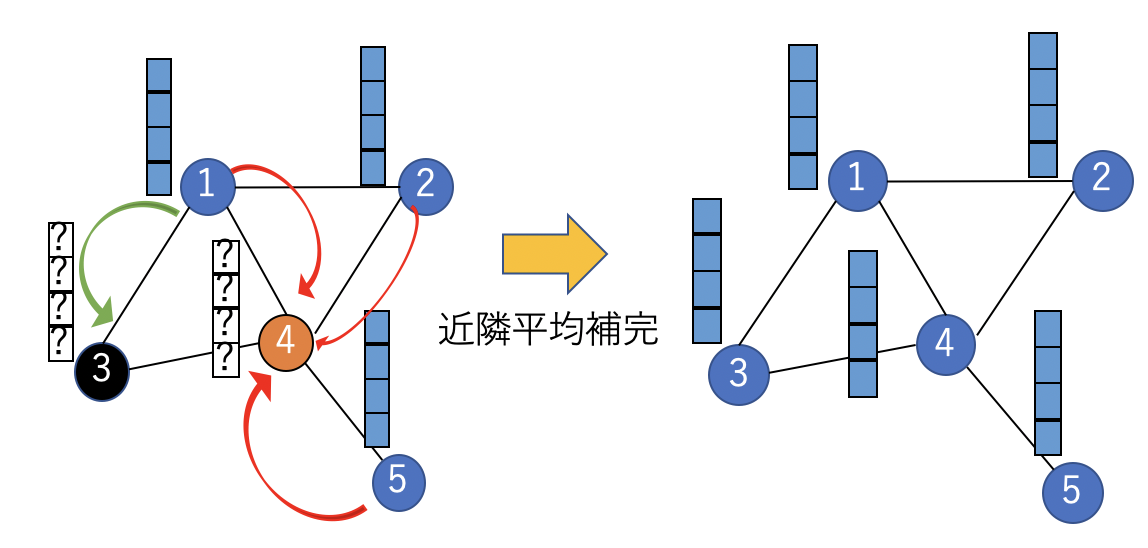
\includegraphics[width=1\hsize]{figures/neighbor_imputation.png}
  \caption{近隣平均補完}
  \label{fig:neighbor_imputation}
\end{figure*}

\section{近隣再帰補完}
本節では提案手法で用いる近隣再帰補完について述べる。近隣再帰補完は構造的補完の1つであり、特徴量の種類ごとに再帰的に補完する手法である。近隣再帰補完は以下の2ステップから成り立っている。
\begin{description}
\item (1)欠損している全ての特徴量を0で埋める
\item (2)元が欠損値であった特徴量だけをそのノードと近隣ノードの特徴量の平均で更新する
\end{description}
近隣再帰補完は(1)で欠損値を0埋めした後に(2)で欠損値の補完を再帰的に決められた回数繰り返す手法である。(2)の特徴量の更新1回で求まる特徴量$X^{(l)}_{ij}$は以下の式\eqref{eq:recursive_imputation}のように定義できる。

\begin{align} \label{eq:recursive_imputation}
    X^{(l)}_{ij} =
    \begin{cases}
      X^{(l-1)}_{ij} & (r_{ij} = 1) \\
      \frac{1}{|N_{i}|}\sum_{k\in{N_{i}}}X^{(l-1)}_{kj} & (r_{ij} = 0)
    \end{cases}
\end{align}

ここで$X^{(l)}_{ij}$は$l$回の再帰後に得られた特徴量であり、$X^{(0)}_{ij} = X_{ij}$と定義する。$N_{i}$はノード$i$の近隣ノードの集合であり、$r_{ij}$は$x_{ij}$が観測値の場合には1で$x_{ij}$が欠損値の場合には0と定義する。

図\ref{fig:recursive_imputation}は近隣再帰補完の例を示している。左図ではノード番号3と4のノードの特徴量が全て欠損しており、ノード番号1,2,5のノードの特徴量は欠損していないケースである。近隣再帰補完を適用することでノード3とノード4の欠損値はまずステップ(1)に従って0で補完される。その後ステップ(2)に従って、元が欠損値であったノードの特徴量は近隣ノードとそのノードの特徴量の平均、つまりノード3はノード1,3,4の特徴量の平均で補完され、ノード4はノード1,2,3,4,5の特徴量の平均で補完される。この(2)の操作を決められた回数行い得られた特徴量を用いてノード3とノード4の欠損値を補完する。

\begin{figure*}[h]
  \centering
  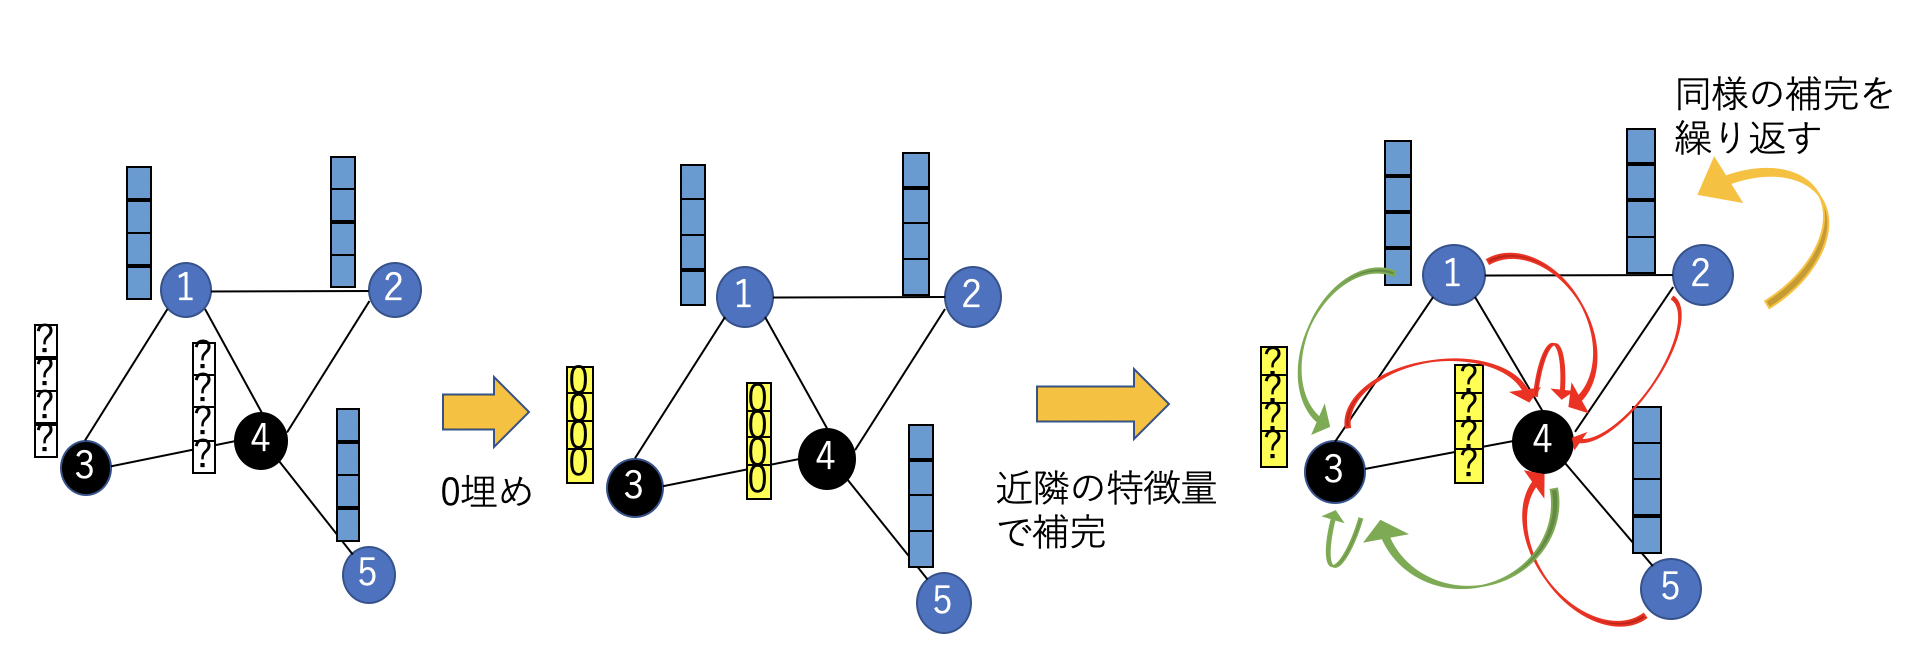
\includegraphics[width=1\hsize]{figures/recursive_imputation.png}
  \caption{近隣再帰補完}
  \label{fig:recursive_imputation}
\end{figure*}

\section{GCN}
提案手法で扱う2層のグラフ畳み込みネットワークについて述べる。1層目の畳み込みネットワークを$GCN_1$、2層目の畳み込みネットワークを$GCN_2$とすると以下の式\eqref{eq:GCN}で表せる。
\begin{eqnarray} \label{eq:GCN}
H_{hid} = GCN_1(X^{'} ,A)\\
H_{out} = GCN_2(H_{hid} ,A)
\end{eqnarray}

ここで、$X^{'}$は欠損値補完により得られた特徴量、$A$は隣接行列、$H_{hid}$はGCN1層目での出力、$H_{out}$はGCN2層目での出力である。

\section{提案手法の定義}
本研究では構造的補完とグラフ畳み込みネットワークを組み合わせたモデルの2つを定義し提案する。提案手法の全体的な流れは図\ref{fig:proposed_models}で示している。1つ目の提案手法GCN\_neighborモデルはまず近隣平均補完で完全データを得た後、MLPを用いて予測するモデルである。2つ目の提案手法GCN\_recursiveモデルはまず近隣再帰補完で完全データを得た後、MLPを用いて予測するモデルである。ここでどちらの提案手法においてもノード分類のタスクにおいてはMLPとして2層GCNを用い、リンク予測のタスクにおいてはVGAEを用いた。ここでVGAEはエンコーダを2層GCN、デコーダを内積とした。
\begin{figure*}[h]
  \centering
  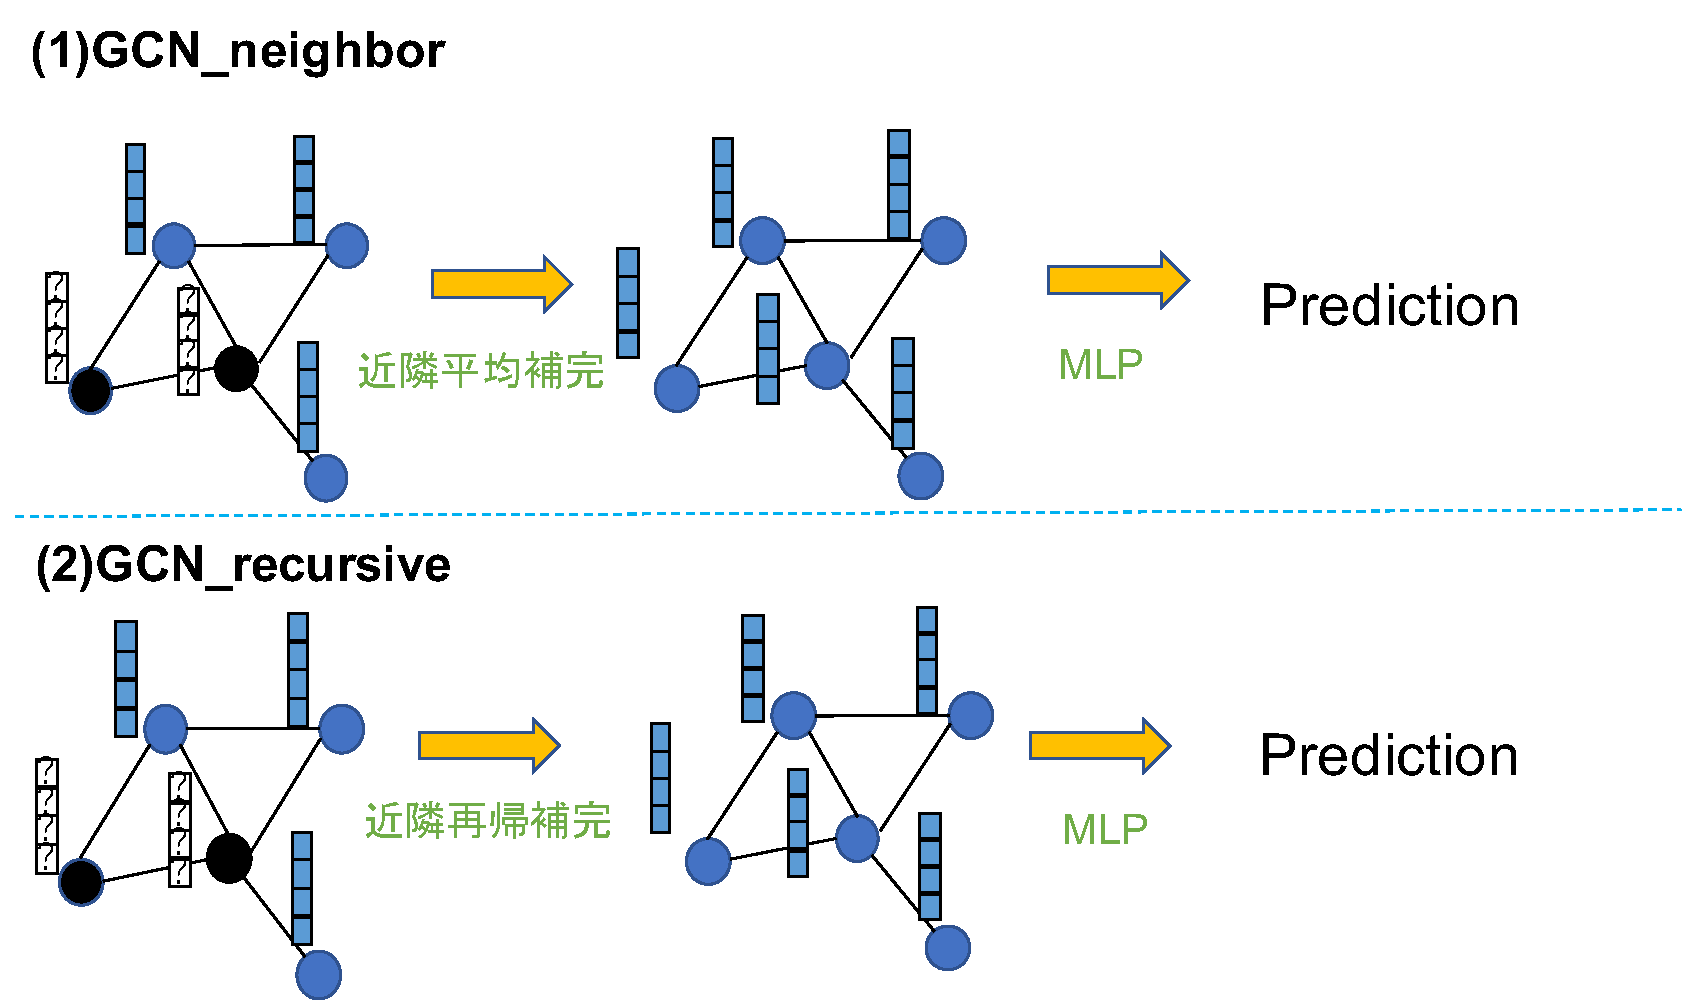
\includegraphics[width=1\hsize]{figures/proposed_architecture.pdf}
  \caption{提案手法の概要}
  \label{fig:proposed_models}
\end{figure*}
